\documentclass[12pt]{article} % For LaTeX2e
\usepackage{nips15submit_e}
\usepackage{times}
%\setmainfont{Times New Roman}
\usepackage{hyperref}
\usepackage{url}
\usepackage{graphicx}
\usepackage{dirtytalk}
\usepackage{float}
\usepackage{color}
\usepackage{amsmath}
%\documentstyle[nips14submit_09,times,art10]{article} % For LaTeX 2.09


\title{Movie Classification Project - Final Report}

\author{
Jiejun Lu, Hongxiang Qiu, Weidong Xu, Zeyu Zhao\\
AC209B Group \#18\\
Harvard University\\
}

\newcommand{\plh}{\textbf{\color{red} PLACEHOLDER }}
\nipsfinalcopy % Uncomment for camera-ready version

\begin{document}

\maketitle

\section{Problem Statement and Motivation}

In this project, we implemented several machine learning models to classify genres of movies using their {\bf overview descriptions and posters}. We further compared those models and made a machine learning pipeline for the best model.

Our pipeline can be used to automatically tag the genres of movies on movie-hosting websites like Netflix and movie-database websites like TMDB.

{\bf All code for scraping data and building the models are submitted with this report.}

\section{Introduction and Description of Data}

In 2016, 736 new movies are released in US cinemas \cite{web_movie_num}, with more on websites like Netflix and YouTube. And the number of new movies released each year is still growing. Therefore, movie genre classification, which helps people quickly find the movies they want to watch, becomes more and more important.

For our project, we built machine learning models to automate the movie genre classification task. The input features for our models are the overview description texts and poster images of a movie and the output is the predicted genres of the given movie.

The first step of building any machine learning model is obtaining the training and test datasets. For this project, we scraped all 361,622 movies from TMDB using the python library {\it tmdbsimple}. As data cleaning, we removed movies with short overview length (less than 10 words) since the majority of them are empty/'No Overview'/'Not found'/ etc., or not enough to describe the movie. We also removed movies without available posters as we would like to integrate poster information to our final model. We are interested in recent movies, so after data cleaning, we only keep the latest 30,000 movies, including their overview descriptions, poster images and ground truth genres. For TMDB dataset, there are $19$ possible genres in total.

Before building our models, we performed the exploratory data analysis (EDA) and get some noteworthy findings on our data. Fig.~\ref{fig:hist} shows the histogram of the count of movies in corresponding genres. We can see the dataset is unbalanced. And intuitively, a movie can have multiple genres. For example, the well-known {\it Titanic} movie has genres {\it drama, romance and thriller}. Fig.~\ref{fig:co-occurrence} shows how genres appear together. It makes intuitive sense to see certain "exciting" categories group together, including crimes, horror, mystery, thriller, and "uplifting" categories group together, including animation, fantasy, family and adventure.

We also examined whether the overview descriptions and posters can be used to predict genres. Fig.~\ref{fig:poster-dif} below shows posters for a documentary movie (left) and an animation movie (right). We can see their styles are pretty different. Fig.~\ref{fig:word-cloud} shows the word cloud we generated for crime movies (top) and romance movies (bottom). We can see their key words are different ("Crime" v.s. "Love"). Therefore, we believe both the posters and overview descriptions are useful to predict genres of movies.

\begin{figure}[H]
\centering
\begin{minipage}{0.5\textwidth}
  \centering
  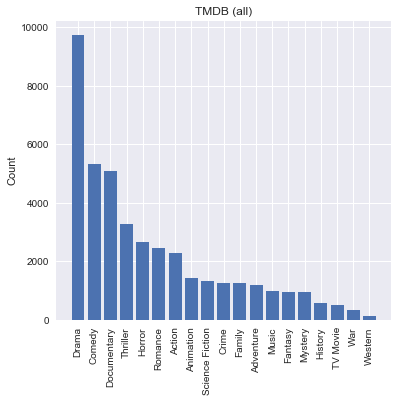
\includegraphics[width=\linewidth]{count.png}
  \caption{Histogram of Movie Genres}
  \label{fig:hist}
\end{minipage}%
\begin{minipage}{0.5\textwidth}
  \centering
  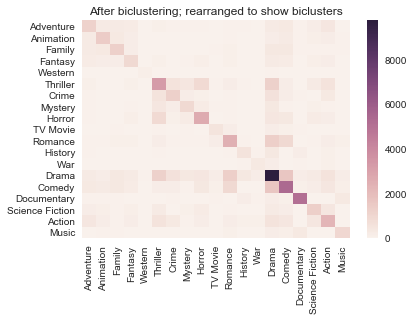
\includegraphics[width=\linewidth,height=7cm]{coappear.png}
  \caption{Co-occurrence of genres}
  \label{fig:co-occurrence}
\end{minipage}%
\end{figure}

\begin{figure}[H]
\centering
\begin{minipage}{0.5\textwidth}
  \centering
  \begin{minipage}{0.5\textwidth}
    \centering
    
\includegraphics[width=0.98\linewidth,height=7cm]{poster.png}
  \end{minipage}%
  \begin{minipage}{0.5\textwidth}
    \centering
    
\includegraphics[width=0.98\linewidth,height=7cm]{poster1.png}
  \end{minipage}%
  \caption{Posters for Different Genres}
  \label{fig:poster-dif}
\end{minipage}%
\begin{minipage}{0.5\textwidth}
  \centering
  \begin{minipage}{\textwidth}
    \centering
    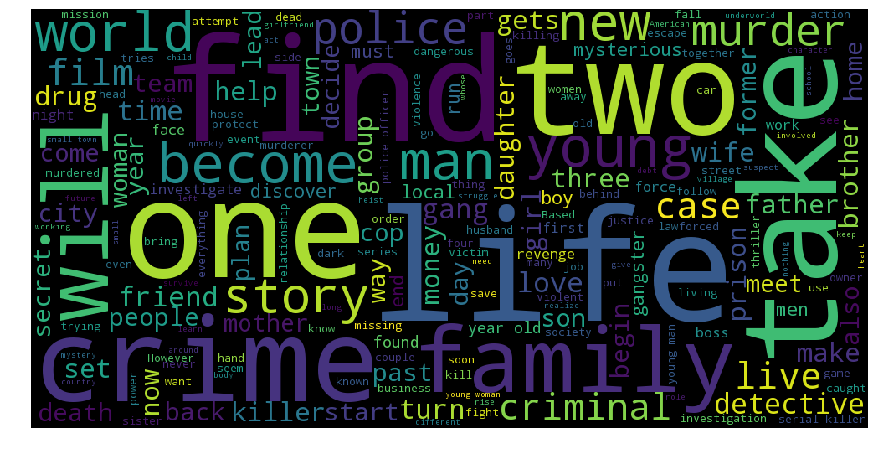
\includegraphics[width=\linewidth]{wordcloud.png}
  \end{minipage}
  \begin{minipage}{\textwidth}
    \centering
    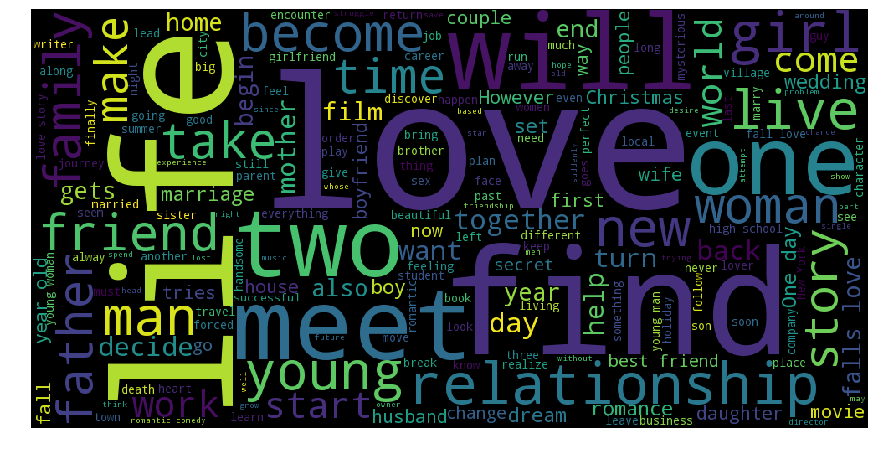
\includegraphics[width=\linewidth]{wordcloud1.png}
  \end{minipage}
  \caption{Word Cloud of Different Genres}
   \label{fig:word-cloud}
\end{minipage}%
\end{figure}

As aforementioned, movie genre classification is a multi-label classification problem. For models solving such problems, evaluation metrics for binary problems can not be easily applied (for example, if using AUC, we will now have $19$ values for all categories instead of $1$, and thus we can't rank our models easily). Previous work \cite{multilabel,multilabel1,multilabel2} uses $F_1$-score (also called $F$-score or $F$-measure) as the evaluation metric. In our project, we choose {\bf micro averaged $F_1$-score} \cite{multilabel} as the metric. We will also report the micro averaged precision and recall. The equations for the three statistics are:

\begin{equation} \label{eq:micro}
\begin{cases}
\text{Precision: }P_{micro}=\frac{\sum_{j=1}^k\sum_{i=1}^nY_i^jZ_i^j}{\sum_{j=1}^k\sum_{i=1}^nZ_i^j}\\
\text{Recall: }R_{micro}=\frac{\sum_{j=1}^k\sum_{i=1}^nY_i^jZ_i^j}{\sum_{j=1}^k\sum_{i=1}^nY_i^j}\\
F_{1-micro} = \frac{2\sum_{j=1}^k\sum_{i=1}^nY_i^jZ_i^j}{\sum_{j=1}^k\sum_{i=1}^nZ_i^j+\sum_{j=1}^k\sum_{i=1}^nY_i^j}
\end{cases}
\end{equation}

$Y_i^j$ in equation~\ref{eq:micro} means \plh By using $F_{1-micro}$ as the single metric, we can easily rank our models.

\section{Related Work}

Overview description texts can be processed with natural language processing (NLP) algorithms. The conventional machine learning method first applies word embedding techniques to data to generate features (typical word representations include bag-of-words, word2vec \cite{word2vec} and GloVE \cite{glove}), and then train classifiers on the generated features. In our project, we will try multinomial naive Bayes and Support Vector Machine (SVM) classifiers.

In recent years, deep learning as shown remarkable  performance in language modeling \plh

Deep learning has also been successful on image classification tasks. So we would like to use convolutional neural networks (CNN) to process posters in our project. However, training a CNN for images from scratch requires (1) a large dataset and (2) a good architecture design. With only 30,000 images, it's not likely we can train a good neural network. As suggested in Stanford CS231n course \cite{transferl}, transfer learning comes to the rescue. Since convolution layers can represent general abstract features of an image, we can fix convolution layers of some pre-trained network and retrain the fully connected layers (or together with last few convolution layers) for our new task. VGG16, VGG19 \cite{vgg} and ResNet-152 \cite{resnet} are well-known CNN architectures for image classification and the pre-trained weights on ImageNet for those architectures are available. We used those three pre-trained network in our project.


\section{Modeling Approach}

\subsection{Baseline Models}
\plh
\subsection{RNN}
\plh
\subsection{CNN}
\plh
\subsection{RNN + CNN}
\plh
\section{Project Trajectory, Results, and Interpretation}

\plh
\section{Conclusions and Possible Future Work}
\plh

\input{bib.bbl}

\end{document}
